\chapter{Experimental Results}

\section{Long Walk Trials}

Figures~\ref{fig:longWalk1_xyz}--\ref{fig:longWalk5_xyz} plot the vehicle's $x$-, $y$-, and $z$-coordinates over time. These plots demonstrate that the UKF's pose estimates were able to track the vehicle's $y$-position accurately over the length of each experimental trial. The plots also show that the UKF pose estimates exhibit some amount of aberrant behavior causing the vehicle's $z$-position to rise the farther the vehicle moves from the origin. The shaded region in Figure~\ref{fig:longWalk1_xyz} clearly highlights this behavior. The vehicle's altitude as estimated by the UKF rises steadily to a maximum of $\sim 1.4$~meters, although in truth the vehicle's altitude was constant throughout. The vehicle's maximum vertical error coincides with its maximal displacement from $\left( 0,\ 0,\ 0 \right)$. 

\begin{figure}
  \centering
    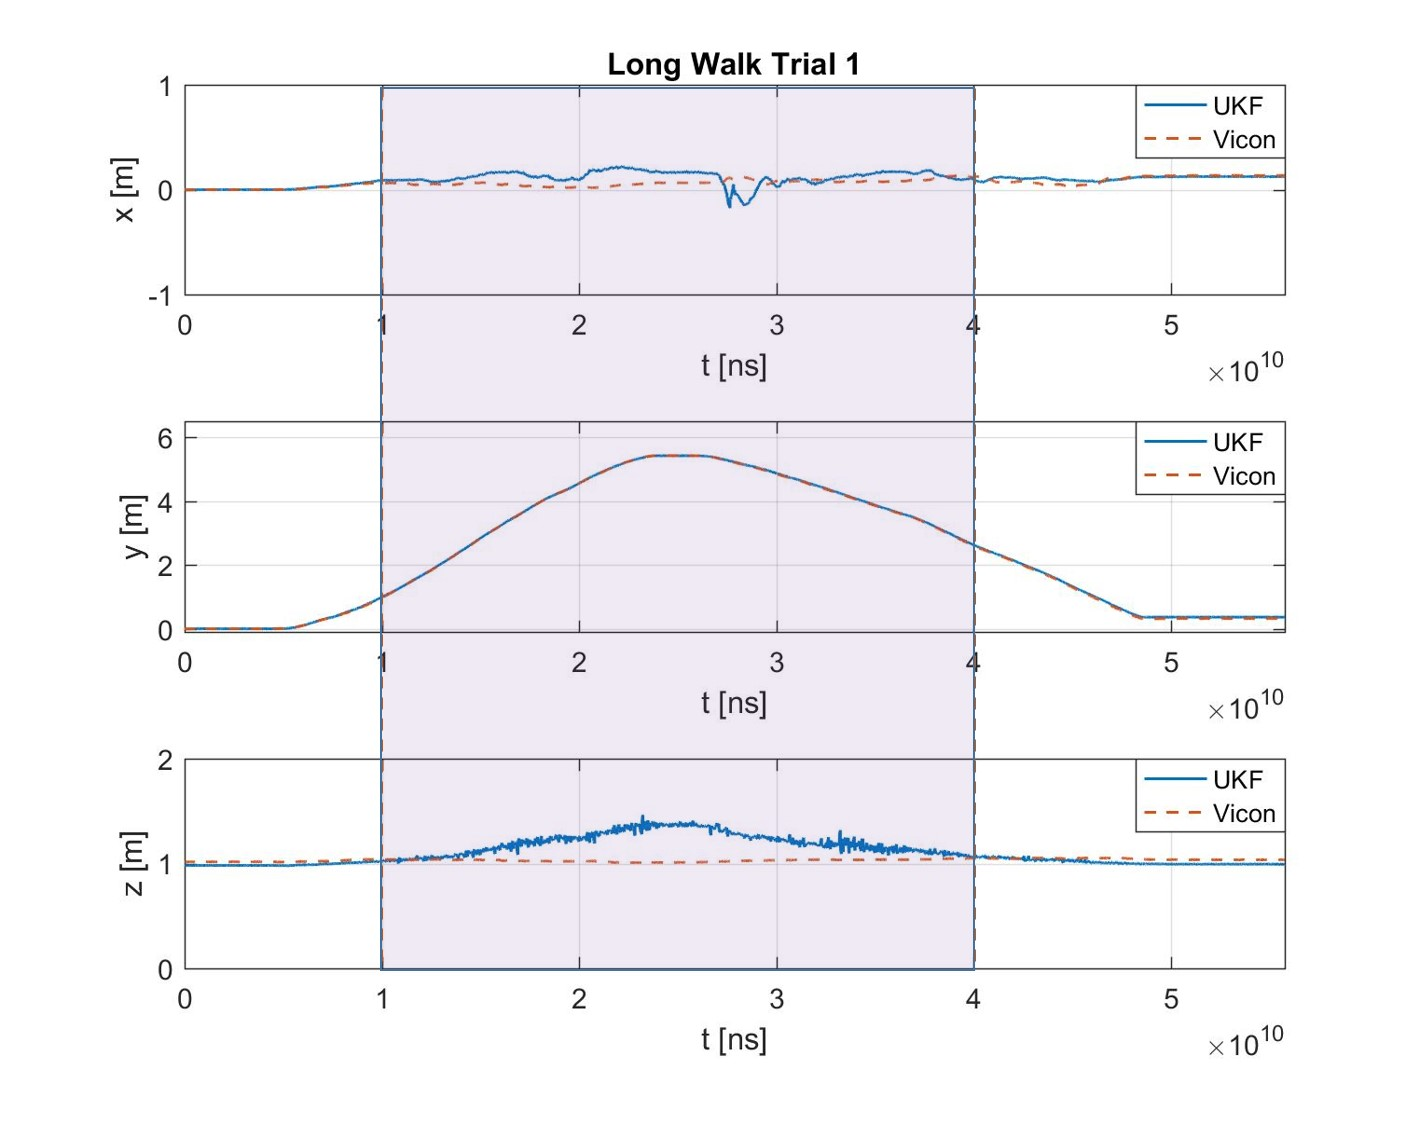
\includegraphics[width=\textwidth]{longWalk1_xyz}
  \caption[Long Walk Trial 1]{Long Walk Trial 1 coordinate plots. The shaded region highlights aberrant behavior coinciding with maximal displacement from the origin.}
  \label{fig:longWalk1_xyz}
\end{figure}

\begin{figure}
  \centering
    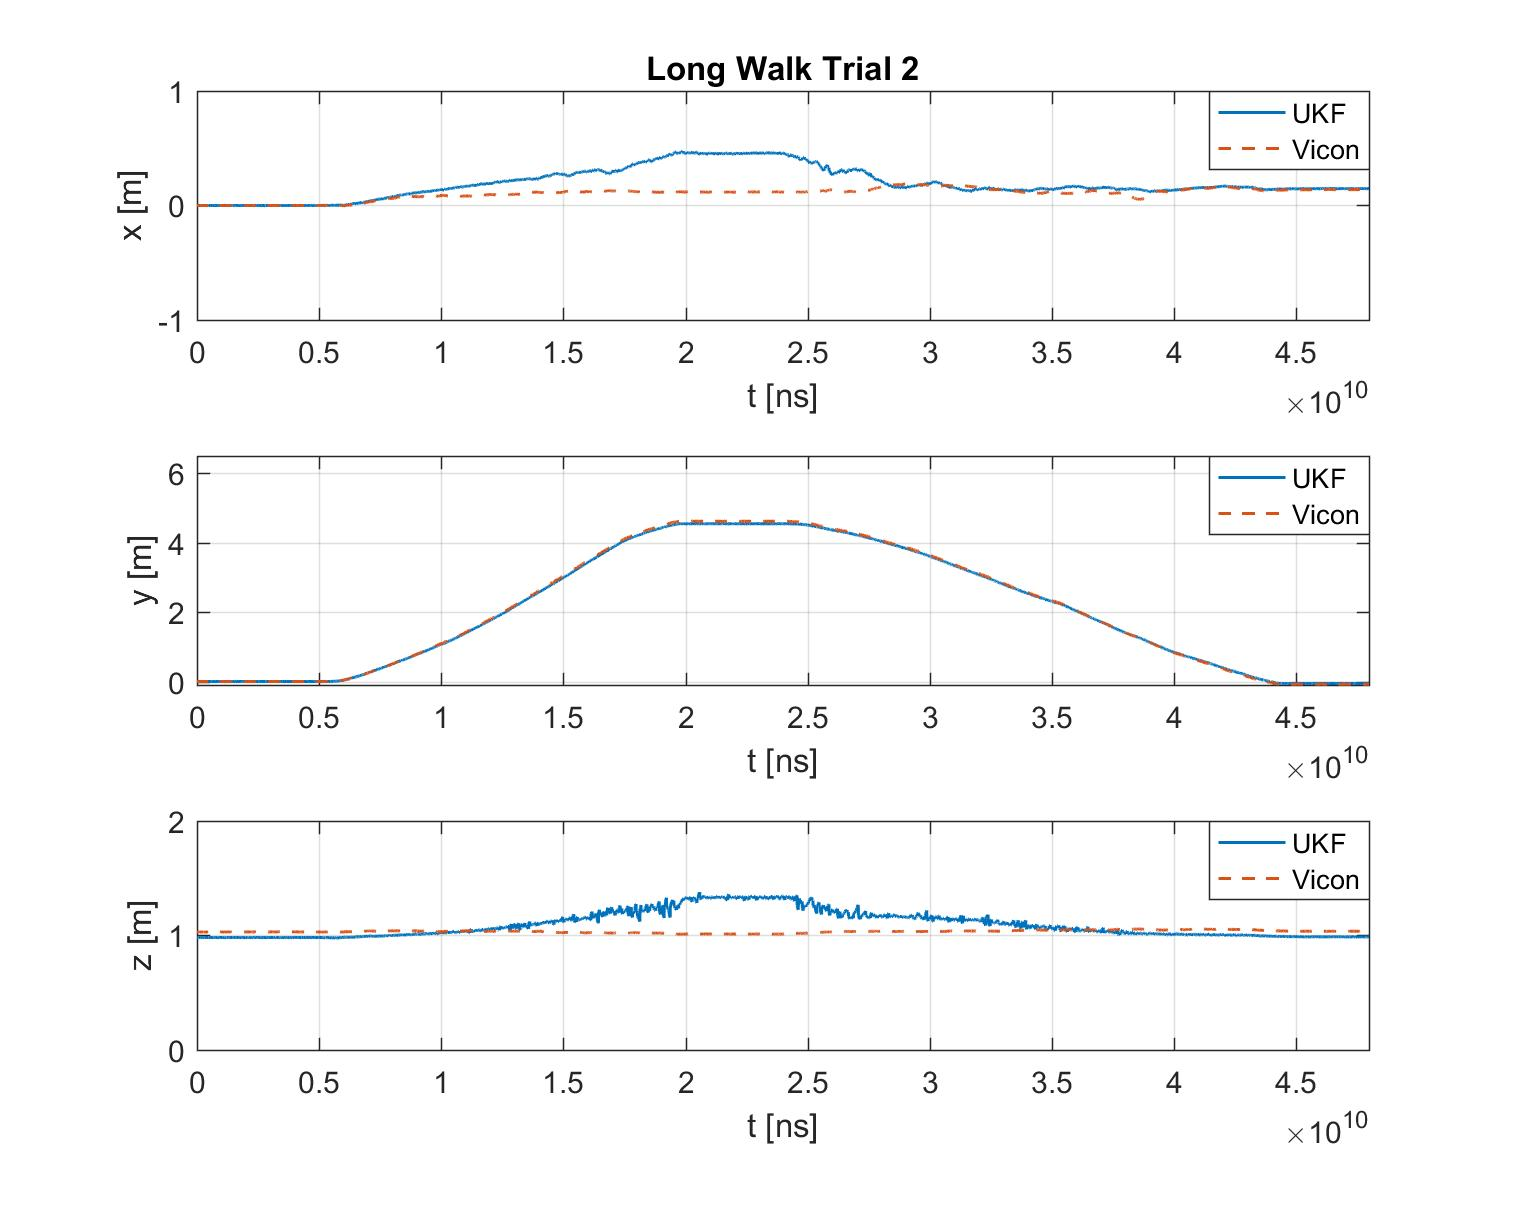
\includegraphics[width=\textwidth]{longWalk2_xyz}
  \caption[Long Walk Trial 2]{Long Walk Trial 2 coordinate plots.}
  \label{fig:longWalk2_xyz}
\end{figure}

\begin{figure}
  \centering
    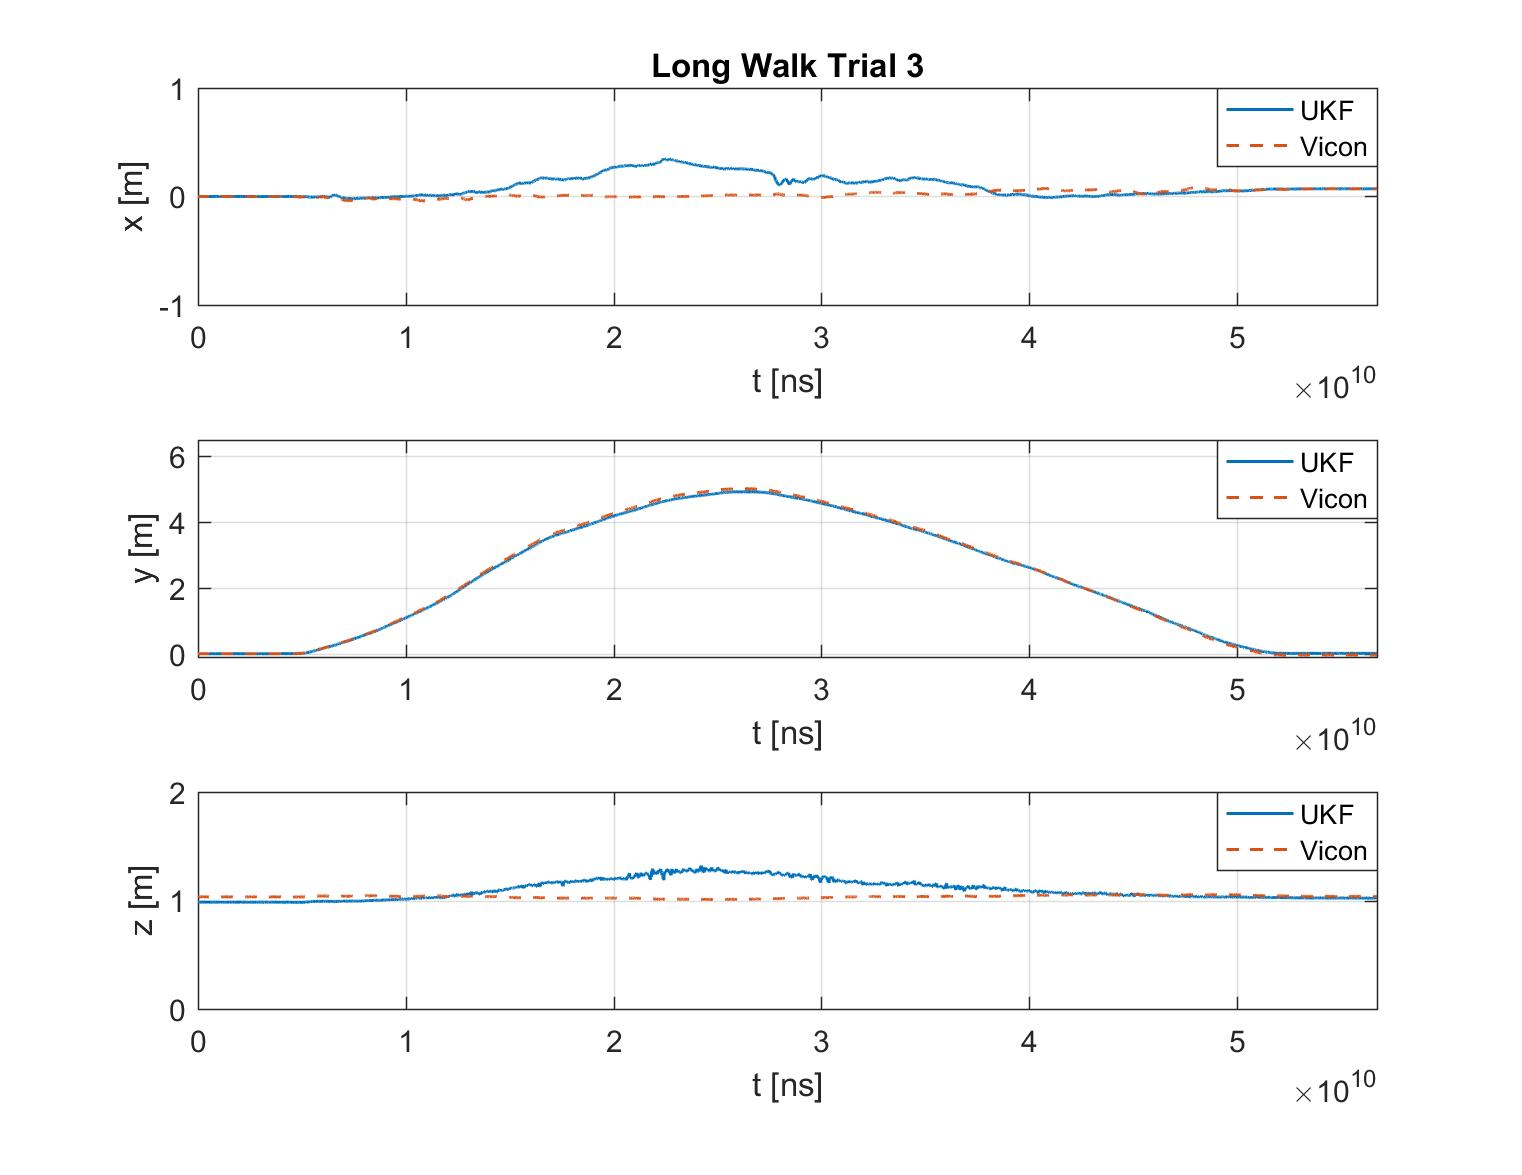
\includegraphics[width=\textwidth]{longWalk3_xyz}
  \caption[Long Walk Trial 3]{Long Walk Trial 3 coordinate plots.}
  \label{fig:longWalk3_xyz}
\end{figure}

\begin{figure}
  \centering
    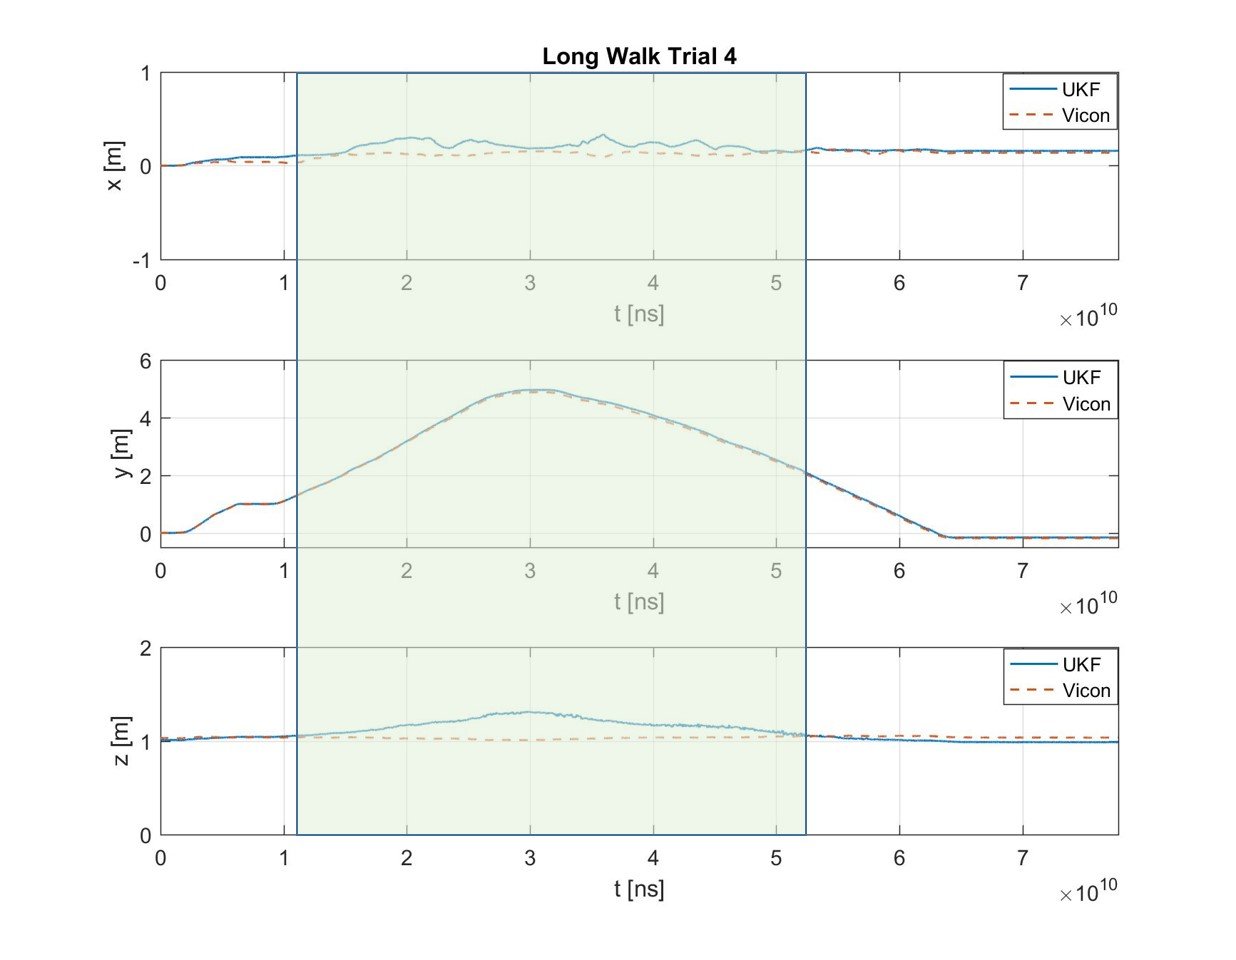
\includegraphics[width=\textwidth]{longWalk4_xyz}
  \caption[Long Walk Trial 4]{Long Walk Trial 4 coordinate plots.}
  \label{fig:longWalk4_xyz}
\end{figure}

\begin{figure}
  \centering
    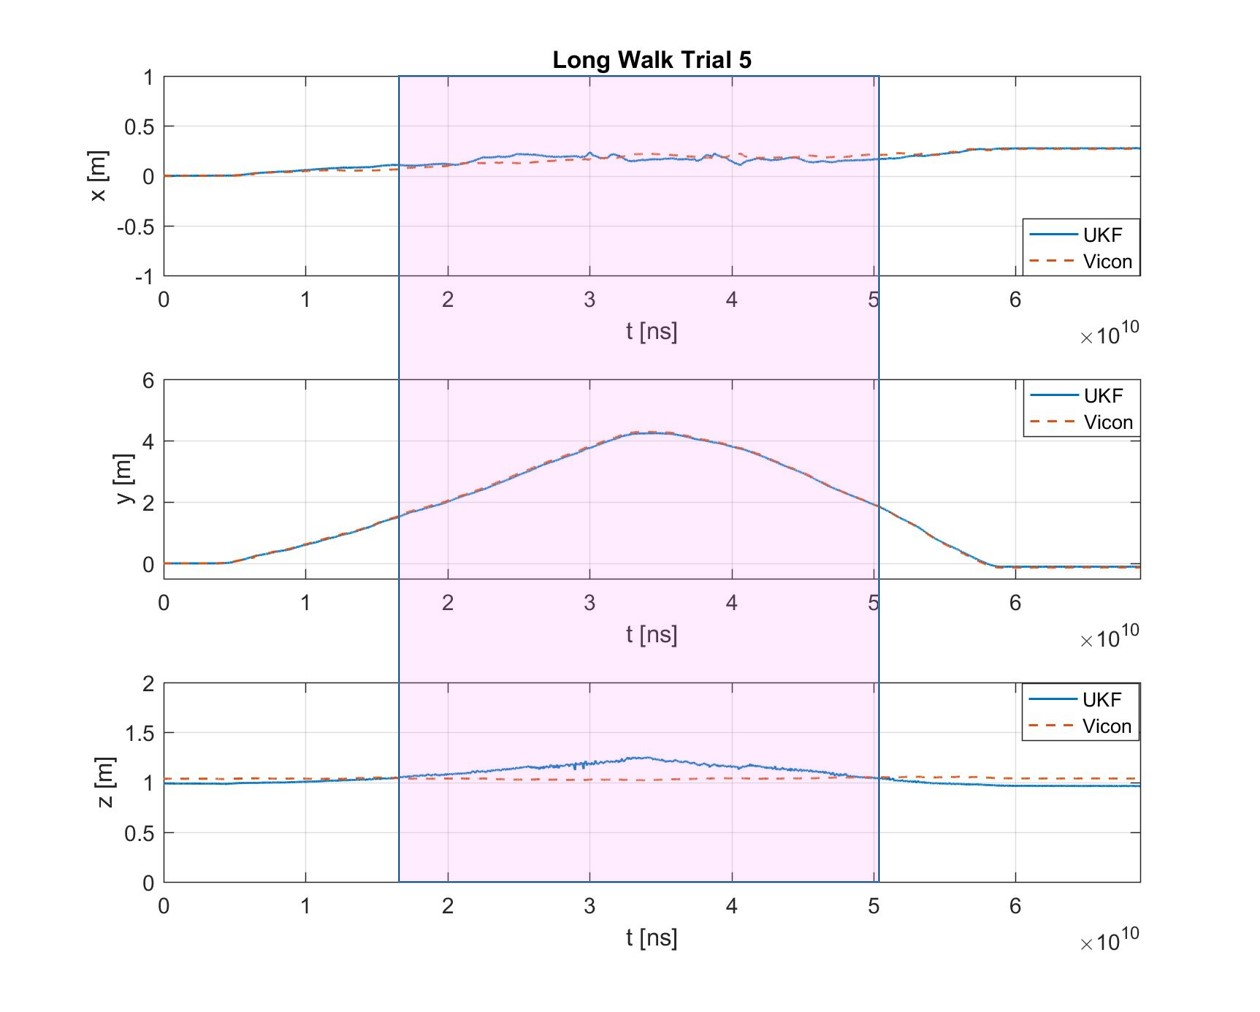
\includegraphics[width=\textwidth]{longWalk5_xyz}
  \caption[Long Walk Trial 5]{Long Walk Trial 5 coordinate plots.}
  \label{fig:longWalk5_xyz}
\end{figure}

\section{Box Pattern Trials}

Figures~\ref{fig:box1_2d}--\ref{fig:box5_3d} plot the estimated and measured trajectories of the vehicle during all five box pattern trials. \todo{more}

\clearpage

% Box 1
\begin{figure}[p]
  \centering
    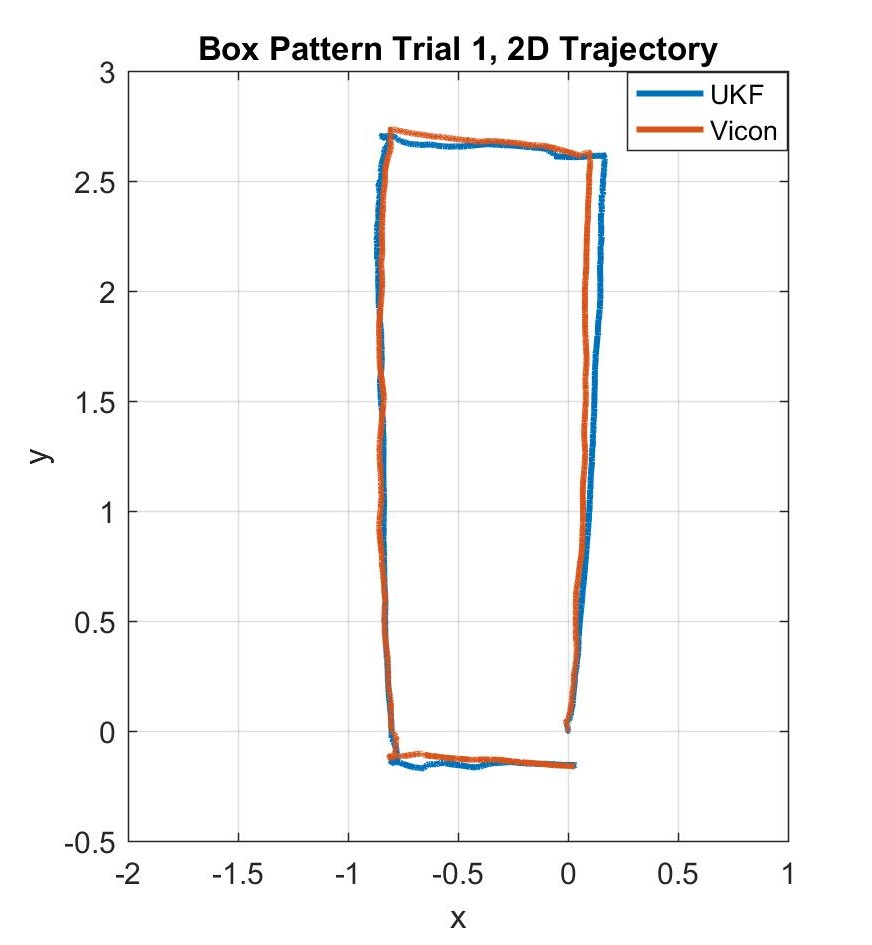
\includegraphics[height=0.6\textwidth]{box1_2d}
  \caption[Box Pattern Trial 1 2D Trajectory]{Box Pattern Trial 1 2D Trajectory.}
  \label{fig:box1_2d}
\end{figure}
\begin{figure}[p]
  \centering
    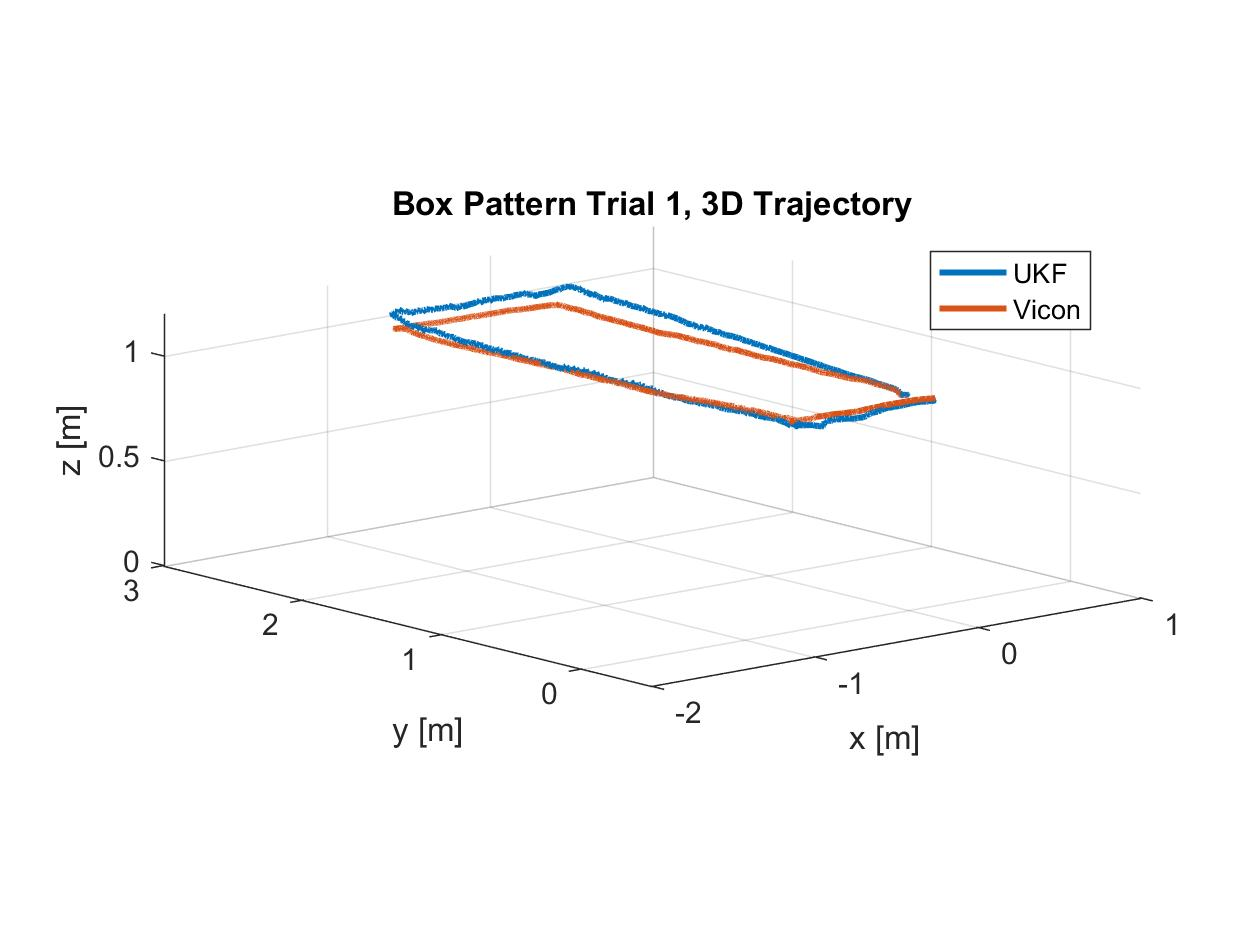
\includegraphics[height=0.7\textwidth]{box1_3d}
  \caption[Box Pattern Trial 1 3D Trajectory]{Box Pattern Trial 1 3D Trajectory.}
  \label{fig:box1_3d}
\end{figure}
\clearpage

% Box 2
\begin{figure}[p]
  \centering
    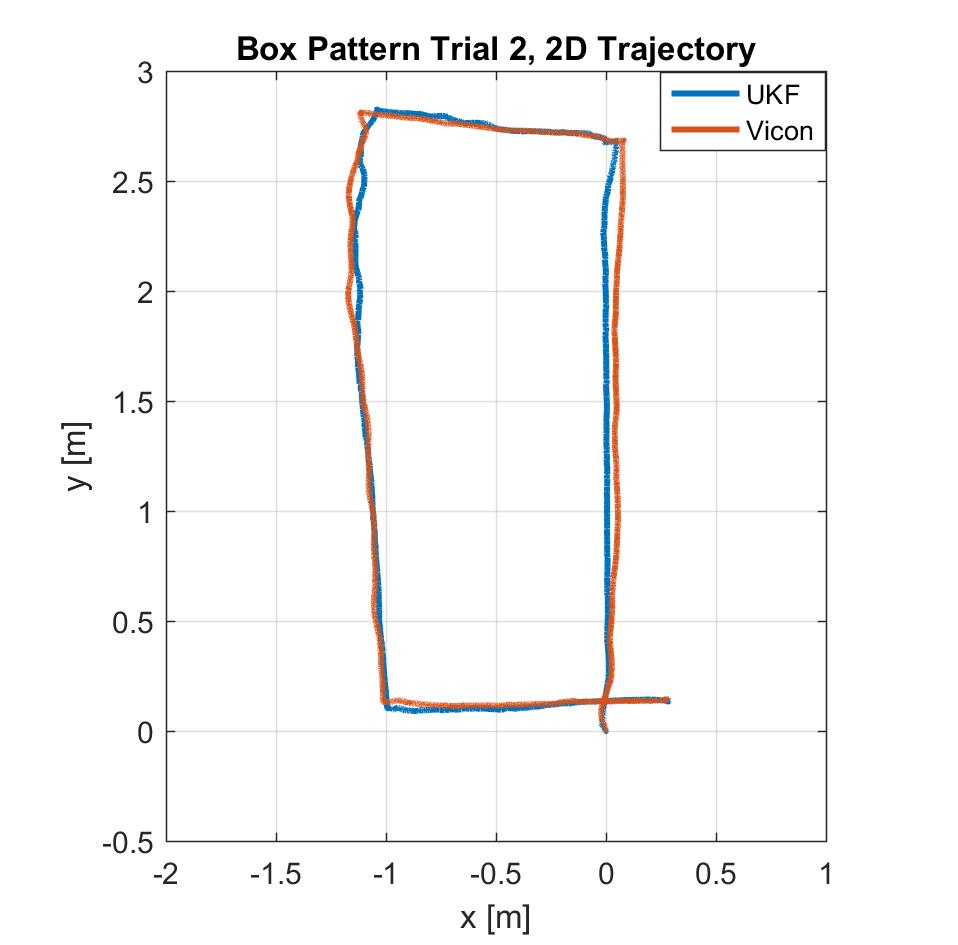
\includegraphics[height=0.6\textwidth]{box2_2d}
  \caption[Box Pattern Trial 2 2D Trajectory]{Box Pattern Trial 2 2D Trajectory.}
  \label{fig:box2_2d}
\end{figure}
\begin{figure}[p]
  \centering
    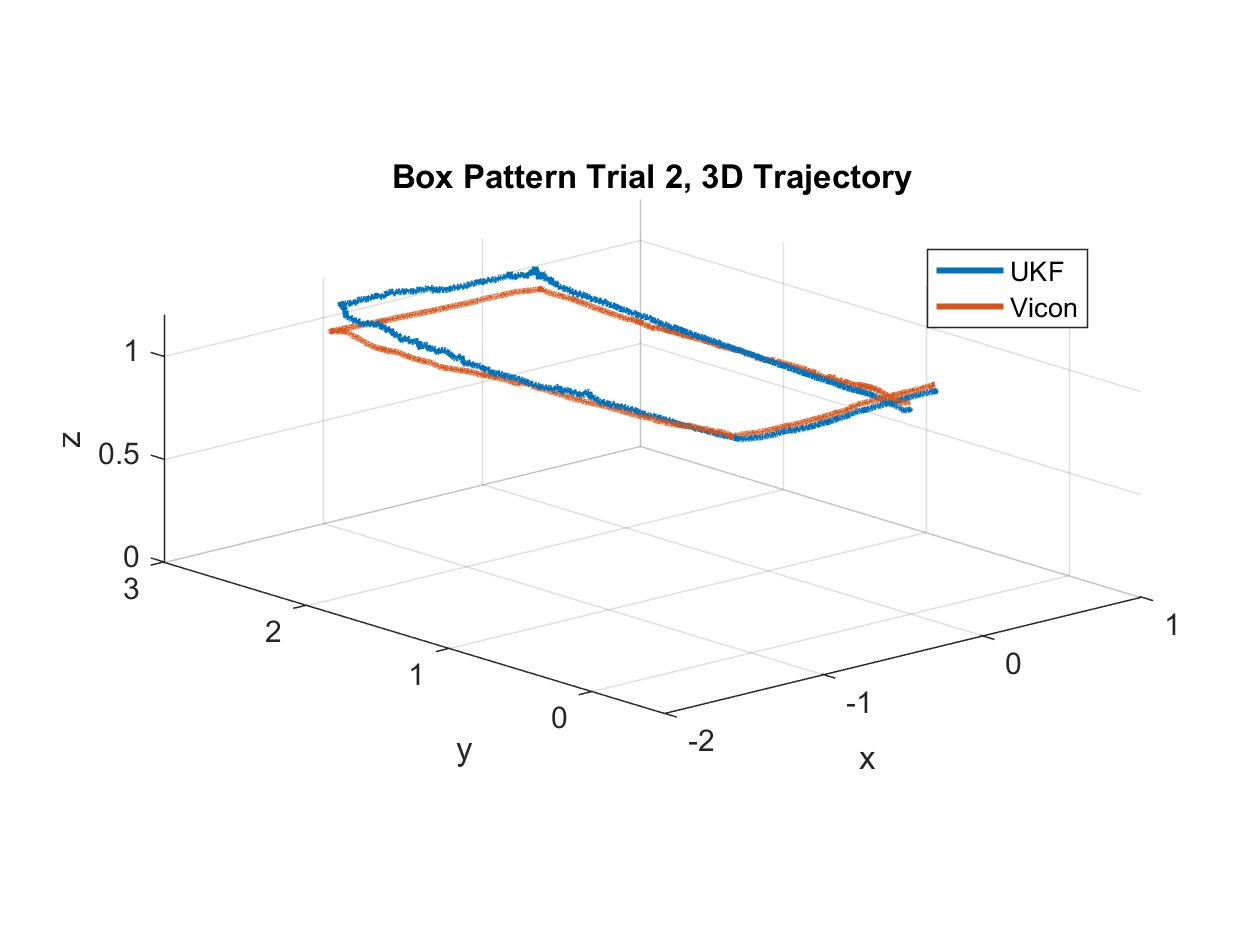
\includegraphics[height=0.7\textwidth]{box2_3d}
  \caption[Box Pattern Trial 2 3D Trajectory]{Box Pattern Trial 2 3D Trajectory.}
  \label{fig:box2_3d}
\end{figure}
\clearpage

% Box 3
\begin{figure}[p]
  \centering
    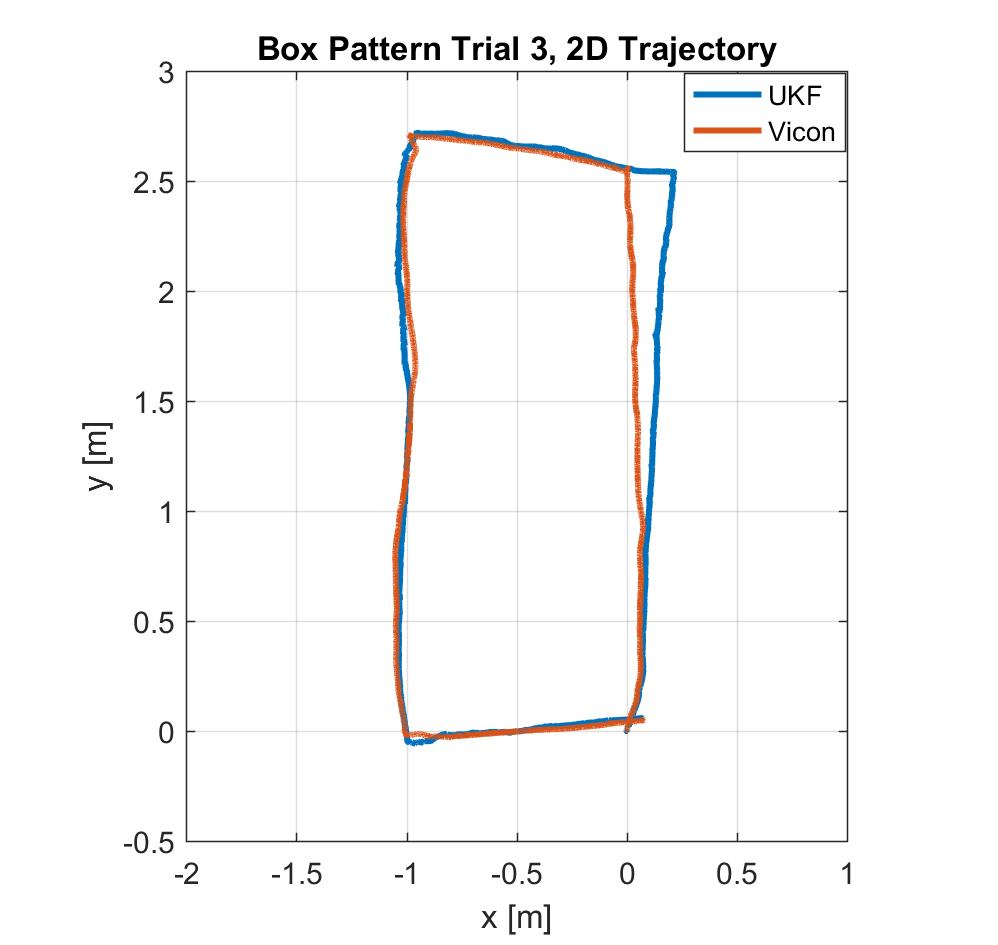
\includegraphics[height=0.6\textwidth]{box3_2d}
  \caption[Box Pattern Trial 3 2D Trajectory]{Box Pattern Trial 3 2D Trajectory.}
  \label{fig:box3_2d}
\end{figure}
\begin{figure}[p]
  \centering
    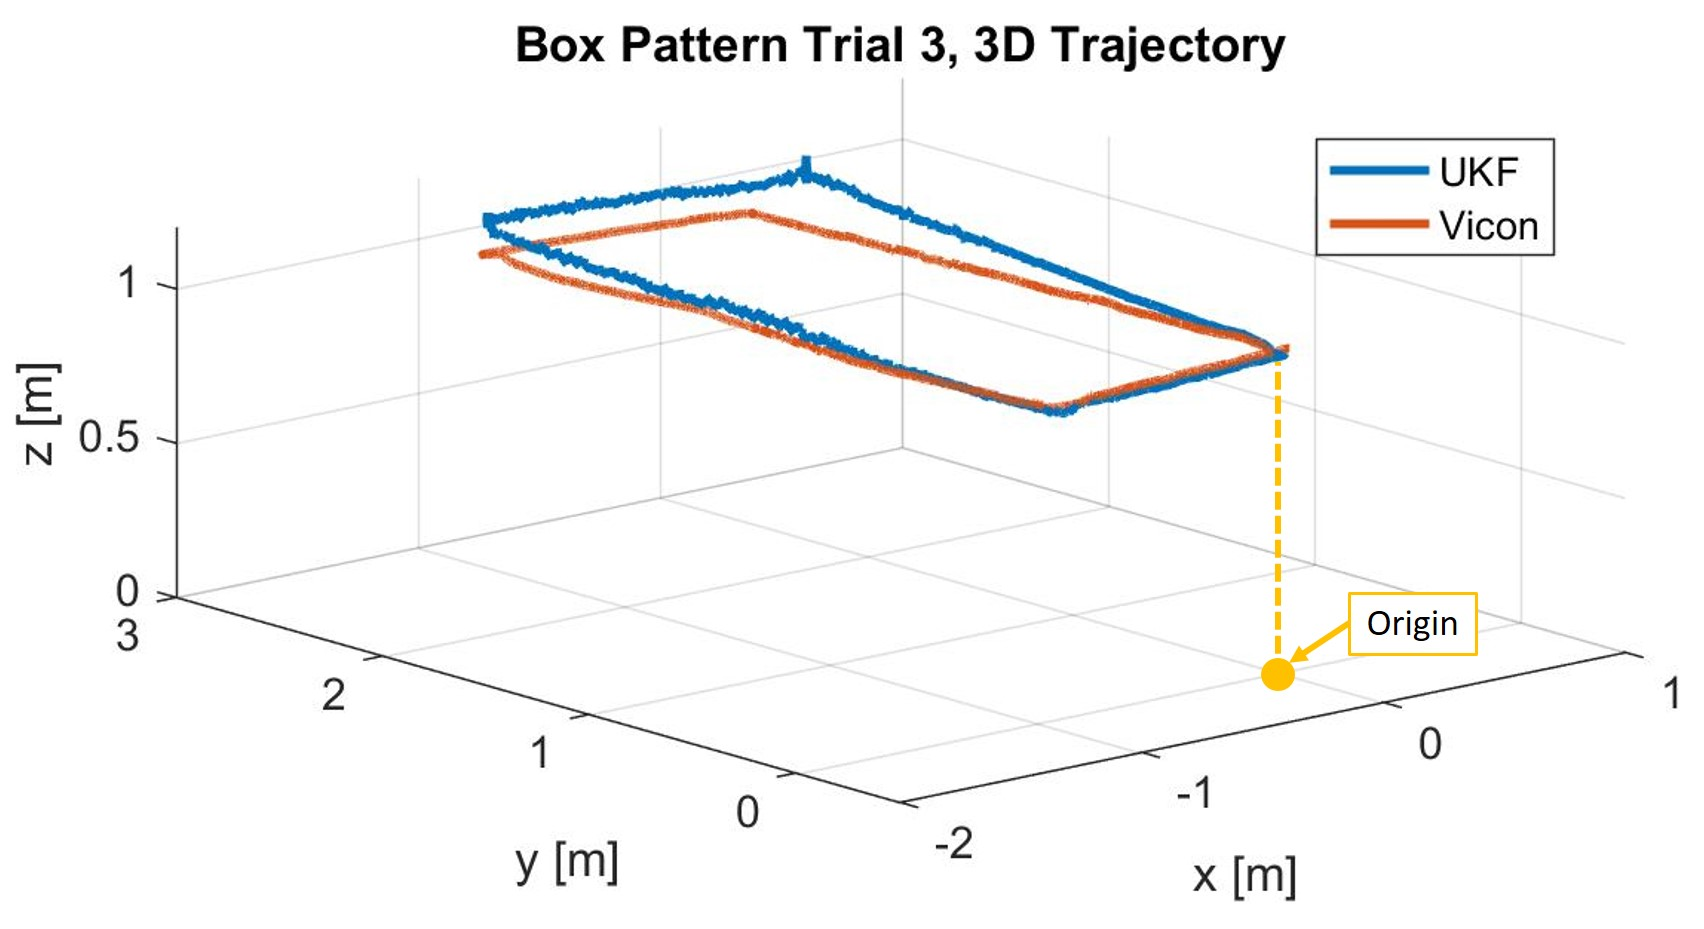
\includegraphics[height=0.7\textwidth]{box3_3d}
  \caption[Box Pattern Trial 3 3D Trajectory]{Box Pattern Trial 3 3D Trajectory.}
  \label{fig:box3_3d}
\end{figure}
\clearpage

% Box 4
\begin{figure}[p]
  \centering
    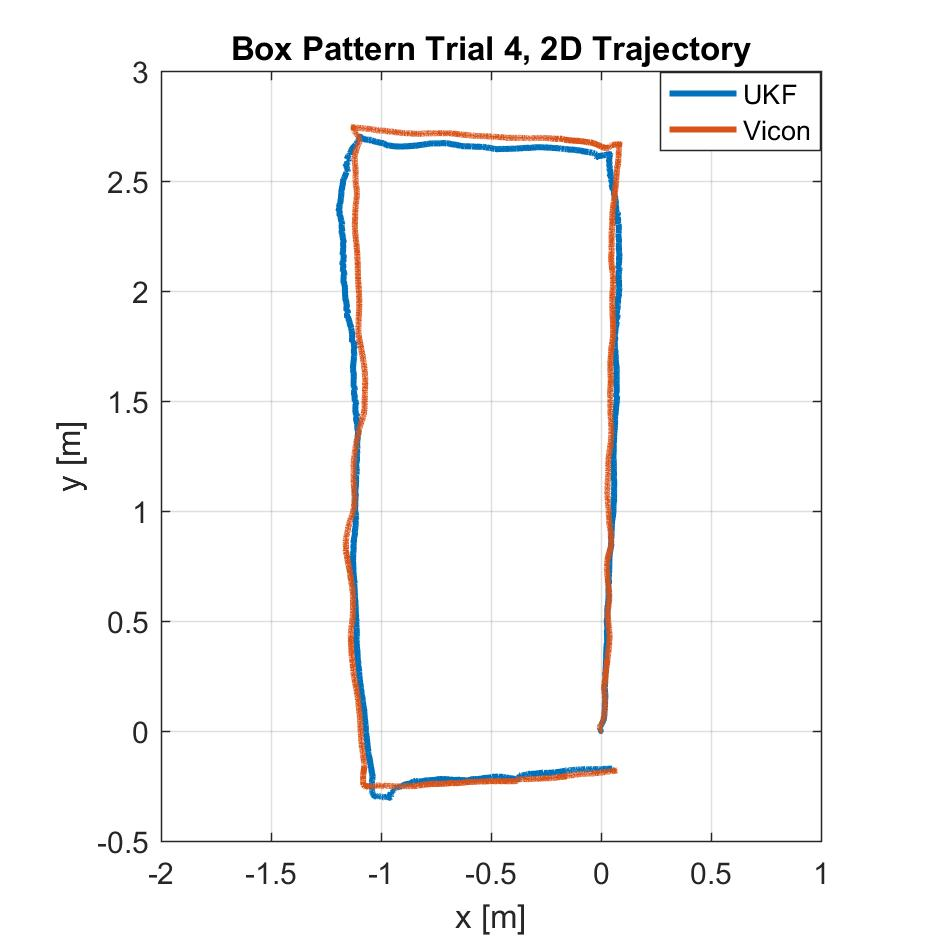
\includegraphics[height=0.6\textwidth]{box4_2d}
  \caption[Box Pattern Trial 4 2D Trajectory]{Box Pattern Trial 4 2D Trajectory.}
  \label{fig:box4_2d}
\end{figure}
\begin{figure}[p]
  \centering
    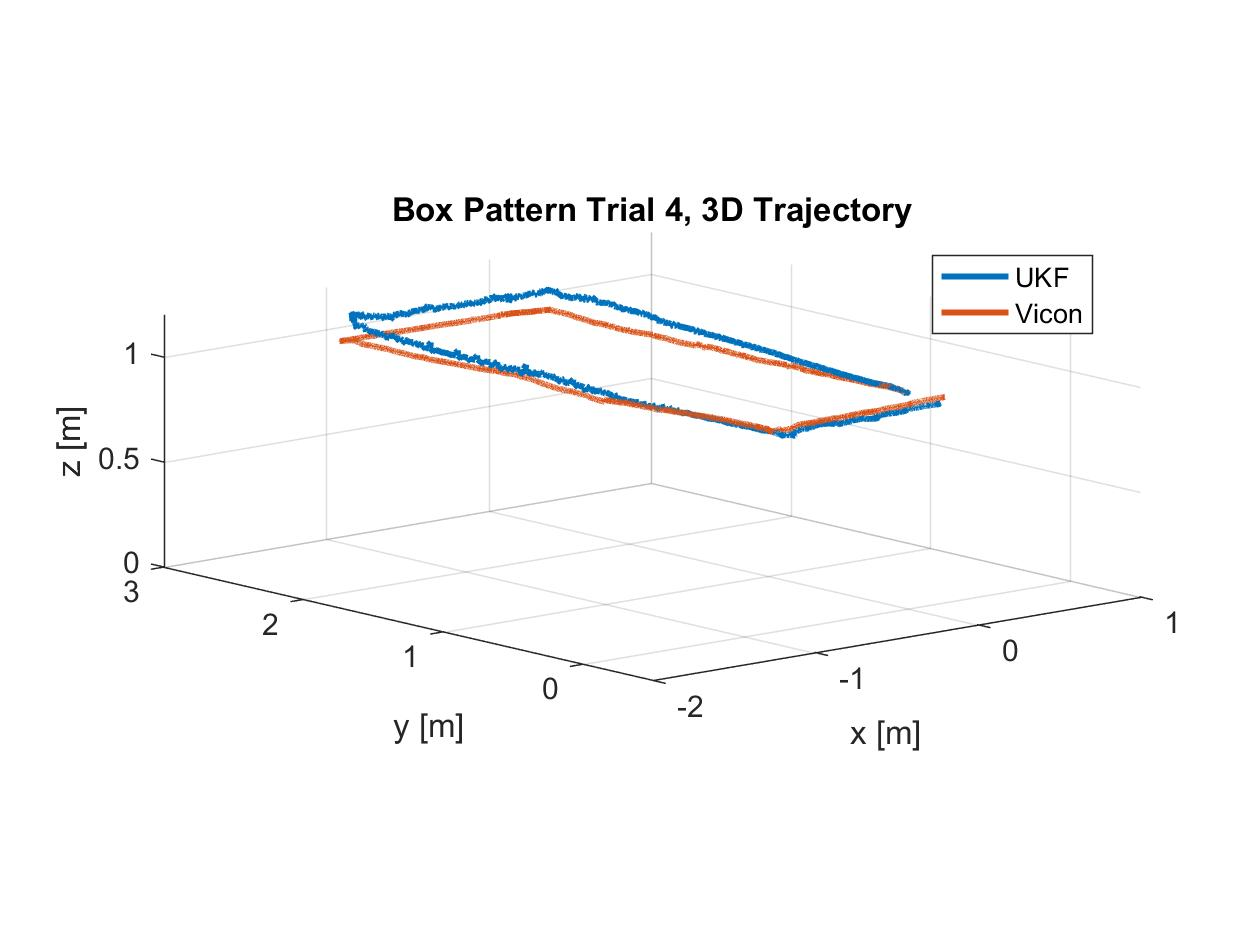
\includegraphics[height=0.7\textwidth]{box4_3d}
  \caption[Box Pattern Trial 4 3D Trajectory]{Box Pattern Trial 4 3D Trajectory.}
  \label{fig:box4_3d}
\end{figure}
\clearpage

% Box 5
\begin{figure}[p]
  \centering
    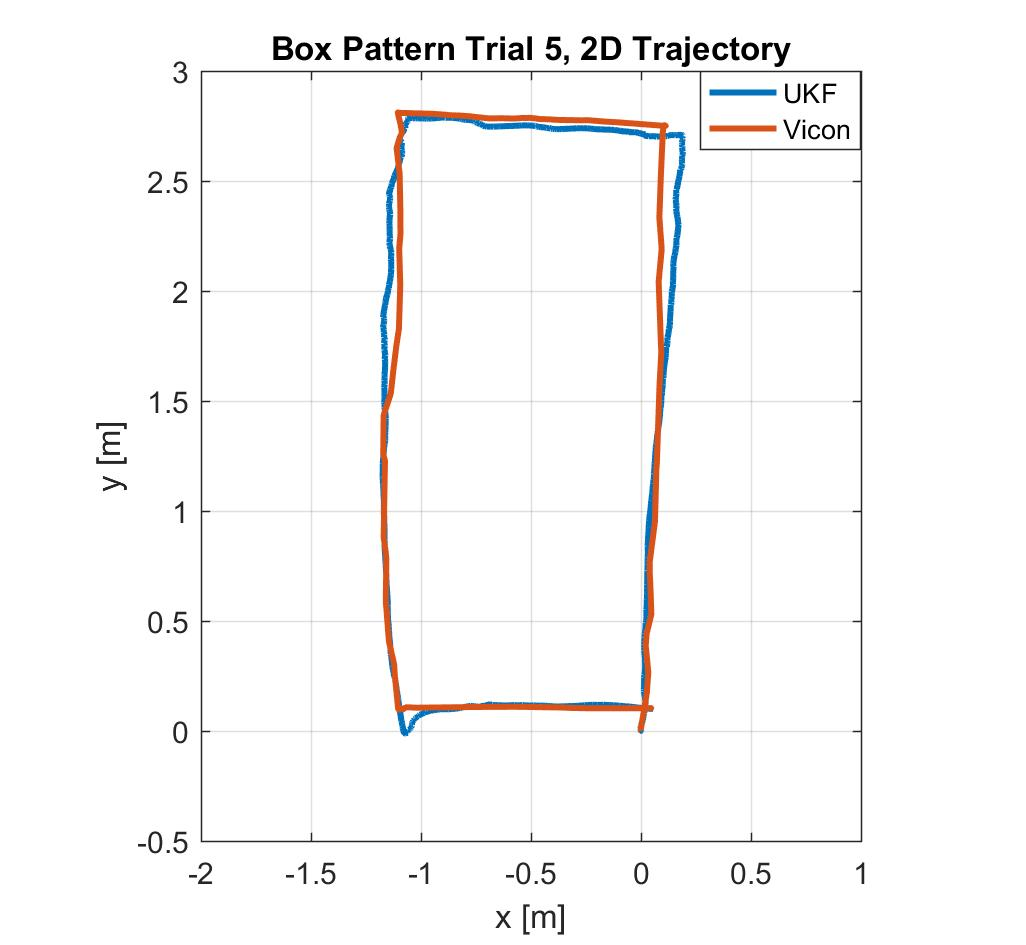
\includegraphics[height=0.6\textwidth]{box5_2d}
  \caption[Box Pattern Trial 5 2D Trajectory]{Box Pattern Trial 5 2D Trajectory.}
  \label{fig:box5_2d}
\end{figure}
\begin{figure}[p]
  \centering
    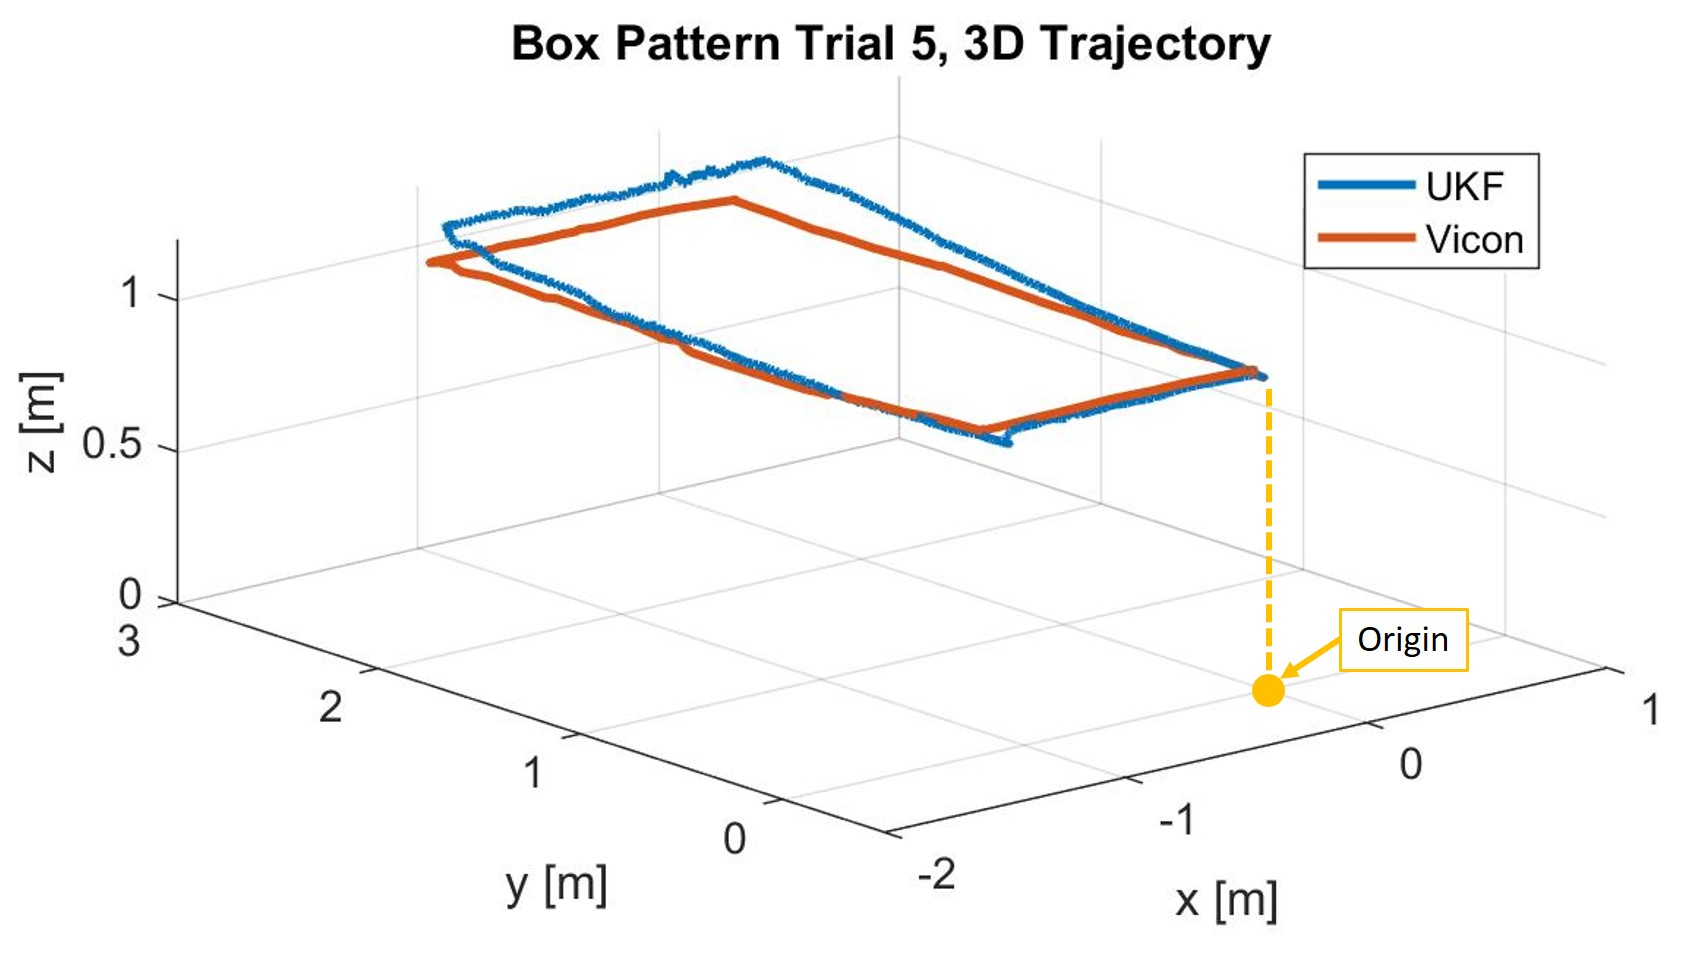
\includegraphics[height=0.7\textwidth]{box5_3d}
  \caption[Box Pattern Trial 5 3D Trajectory]{Box Pattern Trial 5 3D Trajectory.}
  \label{fig:box5_3d}
\end{figure}
\clearpage

